\subsection{Research papers}

\begin{frame}[t]
    \frametitle{Research papers}
    % \begin{center}
    %     The study of the group of rationales points of an elliptic curve, aimed toward its
    %     application in cryptography, was made in parallel
    %     between N. Koblitz and Victor S. Muller.
    % \end{center}
    \begin{itemize}
        \item Neal Koblitz, \textit{\underline{Elliptic curve cryptosystems}}, 1985 \cite{Koblitz1985}
        \item Victor S. Miller, \textit{\underline{Use of elliptic curve in cryptography}}, 1985
            \cite{miller_use_1985}
    \end{itemize}
\noindents
\begin{minipage}[t]{0.48\textwidth}
\begin{figure}[h]
    \centering
    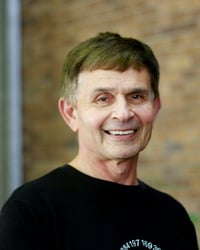
\includegraphics[width=2.5cm, height=3cm]{nealKoblitz}
    {\caption*{Neal Koblitz}}
\end{figure}
\end{minipage}%
\hfill%
\begin{minipage}[t]{0.5\textwidth}
    \begin{figure}[h]
        \centering
        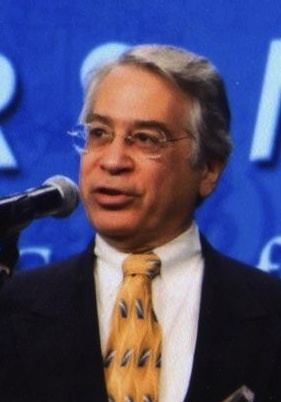
\includegraphics[width=2.5cm, height=3cm]{victorMiller}
        {\caption*{Victor Saul Miller}}
        \label{fig:victorMiller}
    \end{figure}
\end{minipage}
\end{frame}

